\PassOptionsToPackage{table}{xcolor}
\documentclass[aspectratio=169,xcolor=dvipsnames,11pt]{beamer}
\usetheme{SimplePlusAIC}
\usepackage{amsmath}
\usepackage{animate}
\usepackage{hyperref}
\usepackage{cleveref}
\usepackage{caption}
\usepackage{graphicx} % Allows including images
%\usepackage{subfig}
\usepackage{subcaption}
\usepackage{booktabs} % Allows the use of \toprule, \midrule and  \bottomrule in tables
\usepackage{svg} %allows using svg figures
\usepackage{tikz}
\usetikzlibrary{intersections}
\usetikzlibrary{arrows.meta, calc, quotes, tikzmark}
\usepackage{makecell}
\usepackage{multirow}
\usepackage{appendixnumberbeamer}
\usepackage{wrapfig}
\usepackage{verbatim}
\usepackage{tcolorbox}
%\usepackage[dvipsnames]{xcolor}

\usepackage{hhline}
\usepackage{relsize}
\usepackage{bm}
%Select the Epilogue font (requires luaLatex or XeLaTex compilers)
%\setsansfont{Epilogue}[
  %  Path=./epilogueFont/,
  %  Scale=0.9,
  %  Extension = .ttf,
   % UprightFont=*-Regular,
   % BoldFont=*-Bold,
   % ItalicFont=*-Italic,
    %BoldItalicFont=*-BoldItalic
    %]
    \usefonttheme[onlymath]{serif}
% \usepackage{ eulervm } % Euler VM as math serif font

\newcommand*{\defeq}{\stackrel{\text{def}}{=}}
\newcommand{\grad}{\nabla}
\newcommand{\lap}{\Delta}
\newcommand{\weaklyto}{\rightharpoonup}
\newcommand{\weakstar}{\stackrel{*}\rightharpoonup}
\newcommand{\cts}{\hookrightarrow}
\newcommand{\ctsDense}{\xhookrightarrow{d}}
\newcommand{\ctsCompact}{\xhookrightarrow{c}}
\newcommand{\E}{\mathbb{E}}
\newcommand{\pP}{\mathbb{P}}
\newcommand{\R}{\mathbb{R}}
\newcommand{\ER}{\overline{\mathbb{R}}}
\newcommand{\cR}{\mathcal{R}}
\newcommand{\cJ}{\mathcal{J}}
\newcommand{\cG}{\mathcal{G}}
\newcommand{\CVaR}{\textup{CVaR}}
\newcommand{\D}{\textup{ d}}
\newcommand{\dd}{\mathrm{d}}
\newcommand{\fa}{\text{for all }}
\DeclareMathOperator*{\essinf}{\vphantom{p}ess\,inf}
\DeclareMathOperator{\sigmoid}{expit} % a.k.a. logistic sigmoid

\usepackage[ruled,vlined,algo2e]{algorithm2e}
\crefname{algocf}{algorithm}{algorithms}
 \usepackage{caption}

\usepackage{tcolorbox}  % For fancy boxes
\usepackage{lipsum}     % For dummy text

% Define a custom style for the box
\tcbuselibrary{skins, breakable}
\newtcolorbox[auto counter, number within=section]{roundedshadowbox}[2][]{
    colback=white, % Background color (kept white)
    colframe=black, % Border color
    boxrule=0.5pt, % Border thickness
    arc=5mm, % Rounded corners
    shadow=true, % Drop shadow effect
    width=\linewidth, % Full width box
    title=#2, % Title text
    #1 % Additional options (e.g., width override)
}

\usepackage{pgfplots}
\pgfplotsset{compat=1.18}

%\PassOptionsToPackage{table}{xcolor}
%\documentclass[aspectratio=169,xcolor=dvipsnames,11pt]{beamer}
%\usetheme{SimplePlusAIC}
%\usepackage{amsmath}
%\usepackage{hyperref}
%\usepackage{cleveref}
%\usepackage{caption}
%\usepackage{graphicx} % Allows including images
%\usepackage{subcaption}
%\usepackage{booktabs} % Allows the use of \toprule, \midrule and  \bottomrule in tables
%\usepackage{svg} %allows using svg figures
%\usepackage{tikz}
%
%\usepackage{pgfplots}
%\pgfplotsset{compat=1.18}
%
%\usepackage{makecell}
%\usepackage{multirow}
%\usepackage{appendixnumberbeamer}
%\usepackage{wrapfig}
%\usepackage{verbatim}
%\usepackage{tcolorbox}
%\usepackage{hhline}
%\usepackage{relsize}
%\usepackage{bm}
%
%\usefonttheme[onlymath]{serif}
%    
\newcommand{\C}{\mathbb C}

%
%%\font\nullfont=cmr10
%
%\usepackage{tcolorbox}  % For fancy boxes
%\usepackage{lipsum}     % For dummy text
%
%% Define a custom style for the box
%\tcbuselibrary{skins, breakable}
%\newtcolorbox[auto counter, number within=section]{roundedshadowbox}[2][]{
%    colback=white, % Background color (kept white)
%    colframe=black, % Border color
%    boxrule=0.5pt, % Border thickness
%    arc=5mm, % Rounded corners
%    shadow=true, % Drop shadow effect
%    width=\linewidth, % Full width box
%    title=#2, % Title text
%    #1 % Additional options (e.g., width override)
%}


%----------------------------------------------------------------------------------------
%	TITLE PAGE
%----------------------------------------------------------------------------------------

\title[\quad\quad\quad LVPP Course III]{The Latent Variable Proximal Point Method III: Legendre Functions, Applications, and Future Directions
 } % The short title appears at the bottom of every slide, the full title is only on the title page
%\subtitle{Subtitle}

\author{\small{\bf Thomas M. Surowiec}}

\institute[T.M. Surowiec]{Department of Numerical Analysis and Scientific Computing \newline Simula Research Laboratory \newline Oslo, Norway}
% Your institution as it will appear on the bottom of every slide, maybe shorthand to save space


\date[EMS School]{ {\footnotesize 
K\'acov, Czechia, 15-20 June 2025}}
%----------------------------------------------------------------------------------------
%	PRESENTATION SLIDES
%----------------------------------------------------------------------------------------
\begin{document}

{
\setbeamertemplate{background canvas}{}
\frame{\titlepage}
}

\begin{frame}[plain,c]
%\frametitle{A first slide}
\hfill
\begin{center}
\Huge What is really going on here?
\end{center}
\hfill
\end{frame}

\begin{frame}{Overview}

\tableofcontents
\end{frame}


\section{Geometry Preserving Transformations}
\begin{frame}\frametitle{The LVPP Team}
\captionsetup[subfigure]{labelformat=empty}
\begin{figure}
  \begin{subfigure}[b]{2.75cm}
    \includegraphics[width=\linewidth,height=2.5cm, keepaspectratio]{figures/bren096.jpg}
    \caption{Brendan Keith\\ Brown University}
  \end{subfigure}
  \hfill
  \begin{subfigure}[b]{2.75cm}
    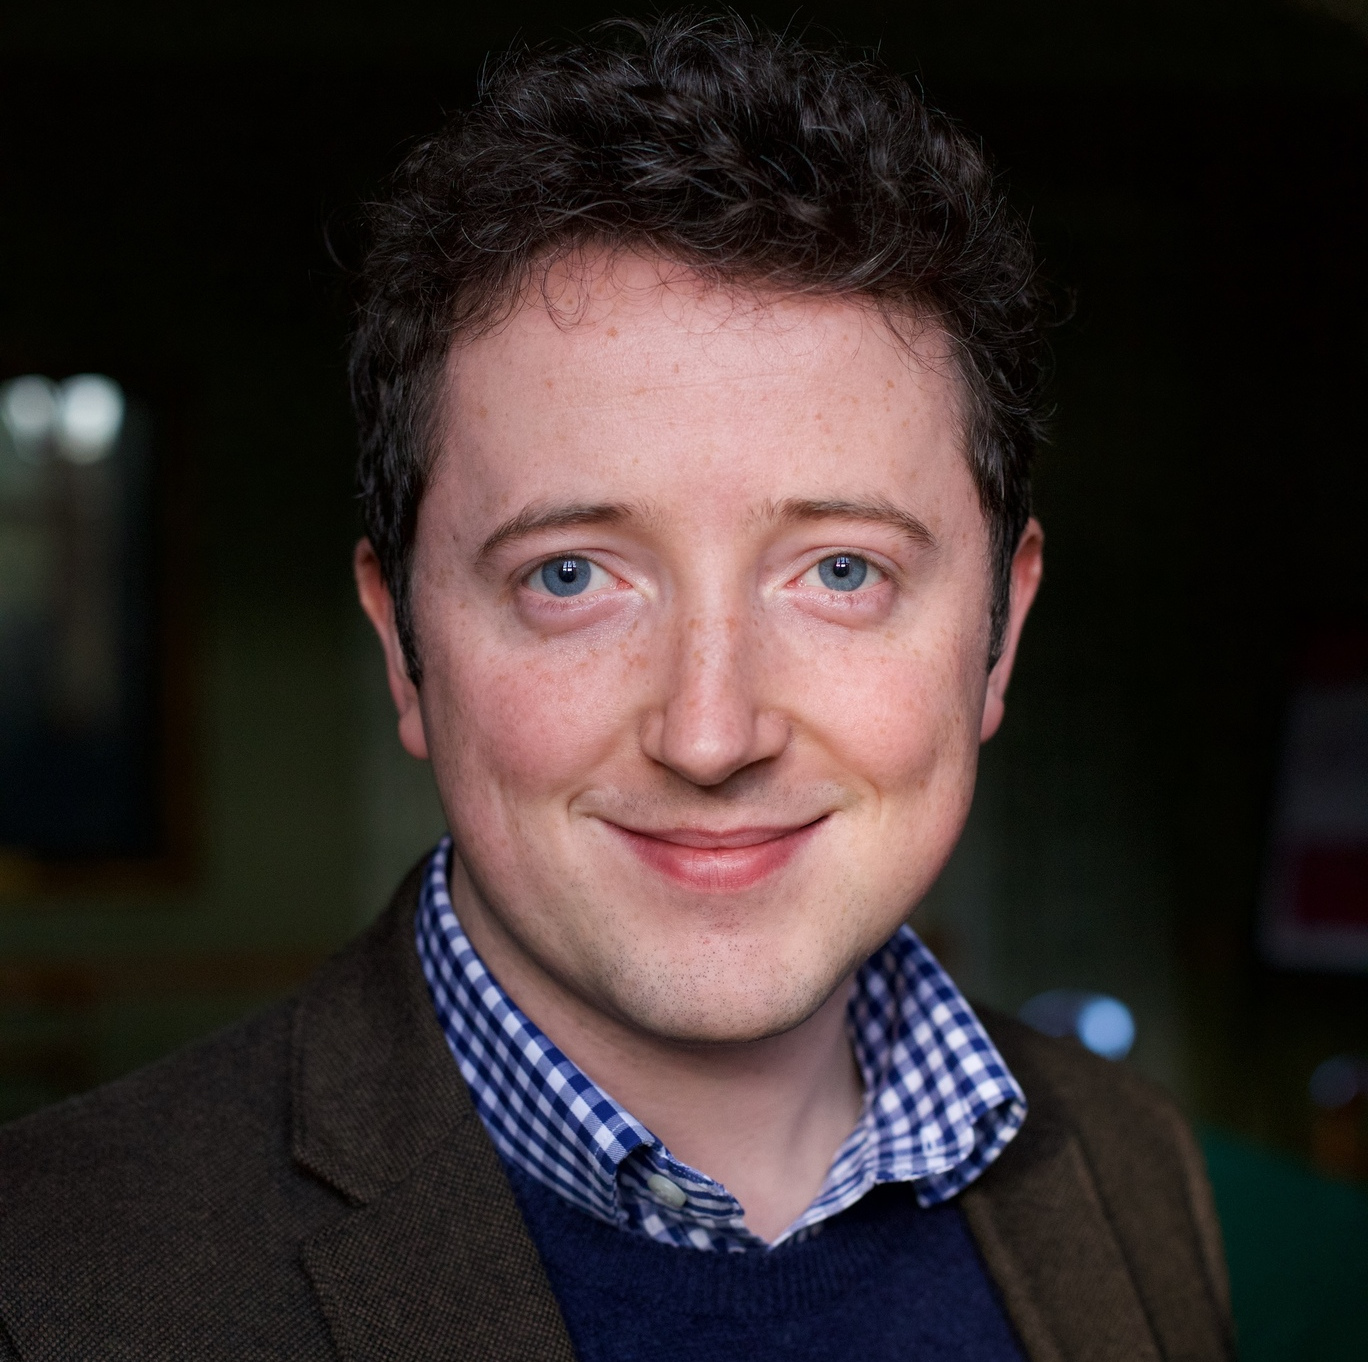
\includegraphics[width=\linewidth,height=2.5cm, keepaspectratio]{figures/patrick.jpg}
    \caption{Patrick E. Farrell\\ Oxford University}
  \end{subfigure}
  \hfill
  \begin{subfigure}[b]{2.75cm}
    
\includegraphics[width=\linewidth,height=2.5cm, keepaspectratio]{figures/joergen.png}
    \caption{Jorgen S. Dokken\\ Simula Research Lab}
  \end{subfigure}
   \hfill
  \begin{subfigure}[b]{3.2cm}
    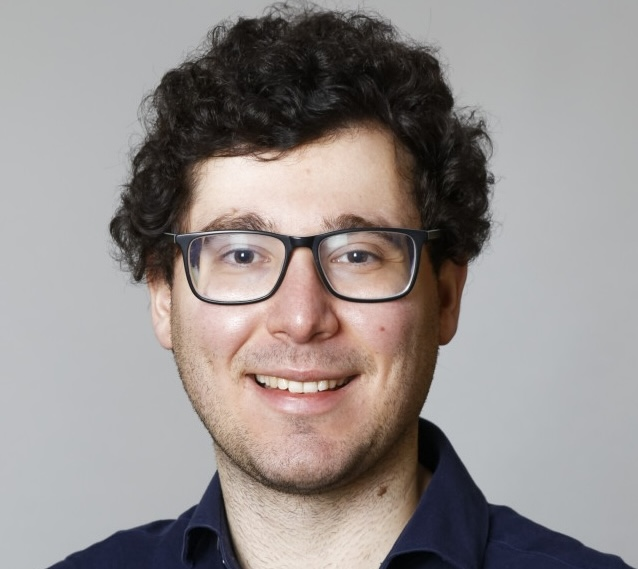
\includegraphics[width=\linewidth,height=2.5cm, keepaspectratio]{figures/papadopoulos.jpg}
    \caption{Ioannis Papadopoulos\\ Weierstra\ss-Institut}
  \end{subfigure}
\hspace{7em}	
%  \hfill
%  \begin{subfigure}[b]{0.19\textwidth}
%    \includegraphics[width=\linewidth]{figures/rivers.jpg}
%    \caption{Diffusive Waves}
%  \end{subfigure}
\end{figure}\vspace{-4ex}
{\tiny
\begin{thebibliography}{1}

\bibitem{BKeith_TMSurowiec_2024}
{\sc B.~Keith and T.M.~Surowiec.}
\newblock Proximal Galerkin: A structure‐preserving finite element method for pointwise bound constraints
\newblock Found. Comut. Math. (2024), \url{https://doi.org/10.1007/s10208-024-09681-8}

\bibitem{JSDokken_etal_2025}
{\sc J.S.~ Dokken, P.E.~Farrell, B.~Keith, I.P.A.~Papadopolous and T.M.~Surowiec.}
\newblock The latent variable proximal point algorithm for variational problems with inequality constraints
\newblock In review (after minor revision) (2025), \url{https://arxiv.org/abs/2503.05672}
\end{thebibliography}
}
\end{frame}

\begin{frame}\frametitle{Bregman Proximal Point}
\only<1,2>{Abstractly speaking, we began with the optimization problem:}
\only<3>{The optimality conditions provide us with a variational inequality:}
\only<4>{Since the variational inequality does not reduce to a variational equation:}
\[
\only<1,2>{ \min_{u \in K} J(u)}
\only<3>{ \min_{u \in K} J(u) \quad \rightarrow \quad \text{Find } u \in K : J'(u)(v - u) \ge 0,\; \forall v \in K.}
\only<4>{\text{ Solve }\quad \min_{u \in K} J(u) \quad \text{ by recursively solving }  \quad \min_{u \in K} J(u) + \alpha^{-1} D(u,u_{\text{old}}) \quad \text{instead.}}
\]
\only<2,3>{
\begin{minipage}{0.5\textwidth}
\begin{beamercolorbox}[rounded=true, shadow=true, wd=\textwidth]{block body}
$V$: a reflexive Banach space,\smallskip

$K \subset V$: a closed convex set,\smallskip

$J$: a smooth coercive functional.
\end{beamercolorbox}
\end{minipage}
}
\only<4->{
\begin{minipage}{0.5\textwidth}
\begin{beamercolorbox}[rounded=true, shadow=true, wd=\textwidth]{block body}
$V$: a reflexive Banach space,\smallskip

$K \subset V$: a closed convex set,\smallskip

$J$: a smooth coercive functional,\smallskip

$D : K \times K \to \overline{\mathbb R}$ is a \alert{Bregman distance.}
\end{beamercolorbox}
\end{minipage}%
\begin{minipage}{0.5\textwidth}
\begin{figure}[h]
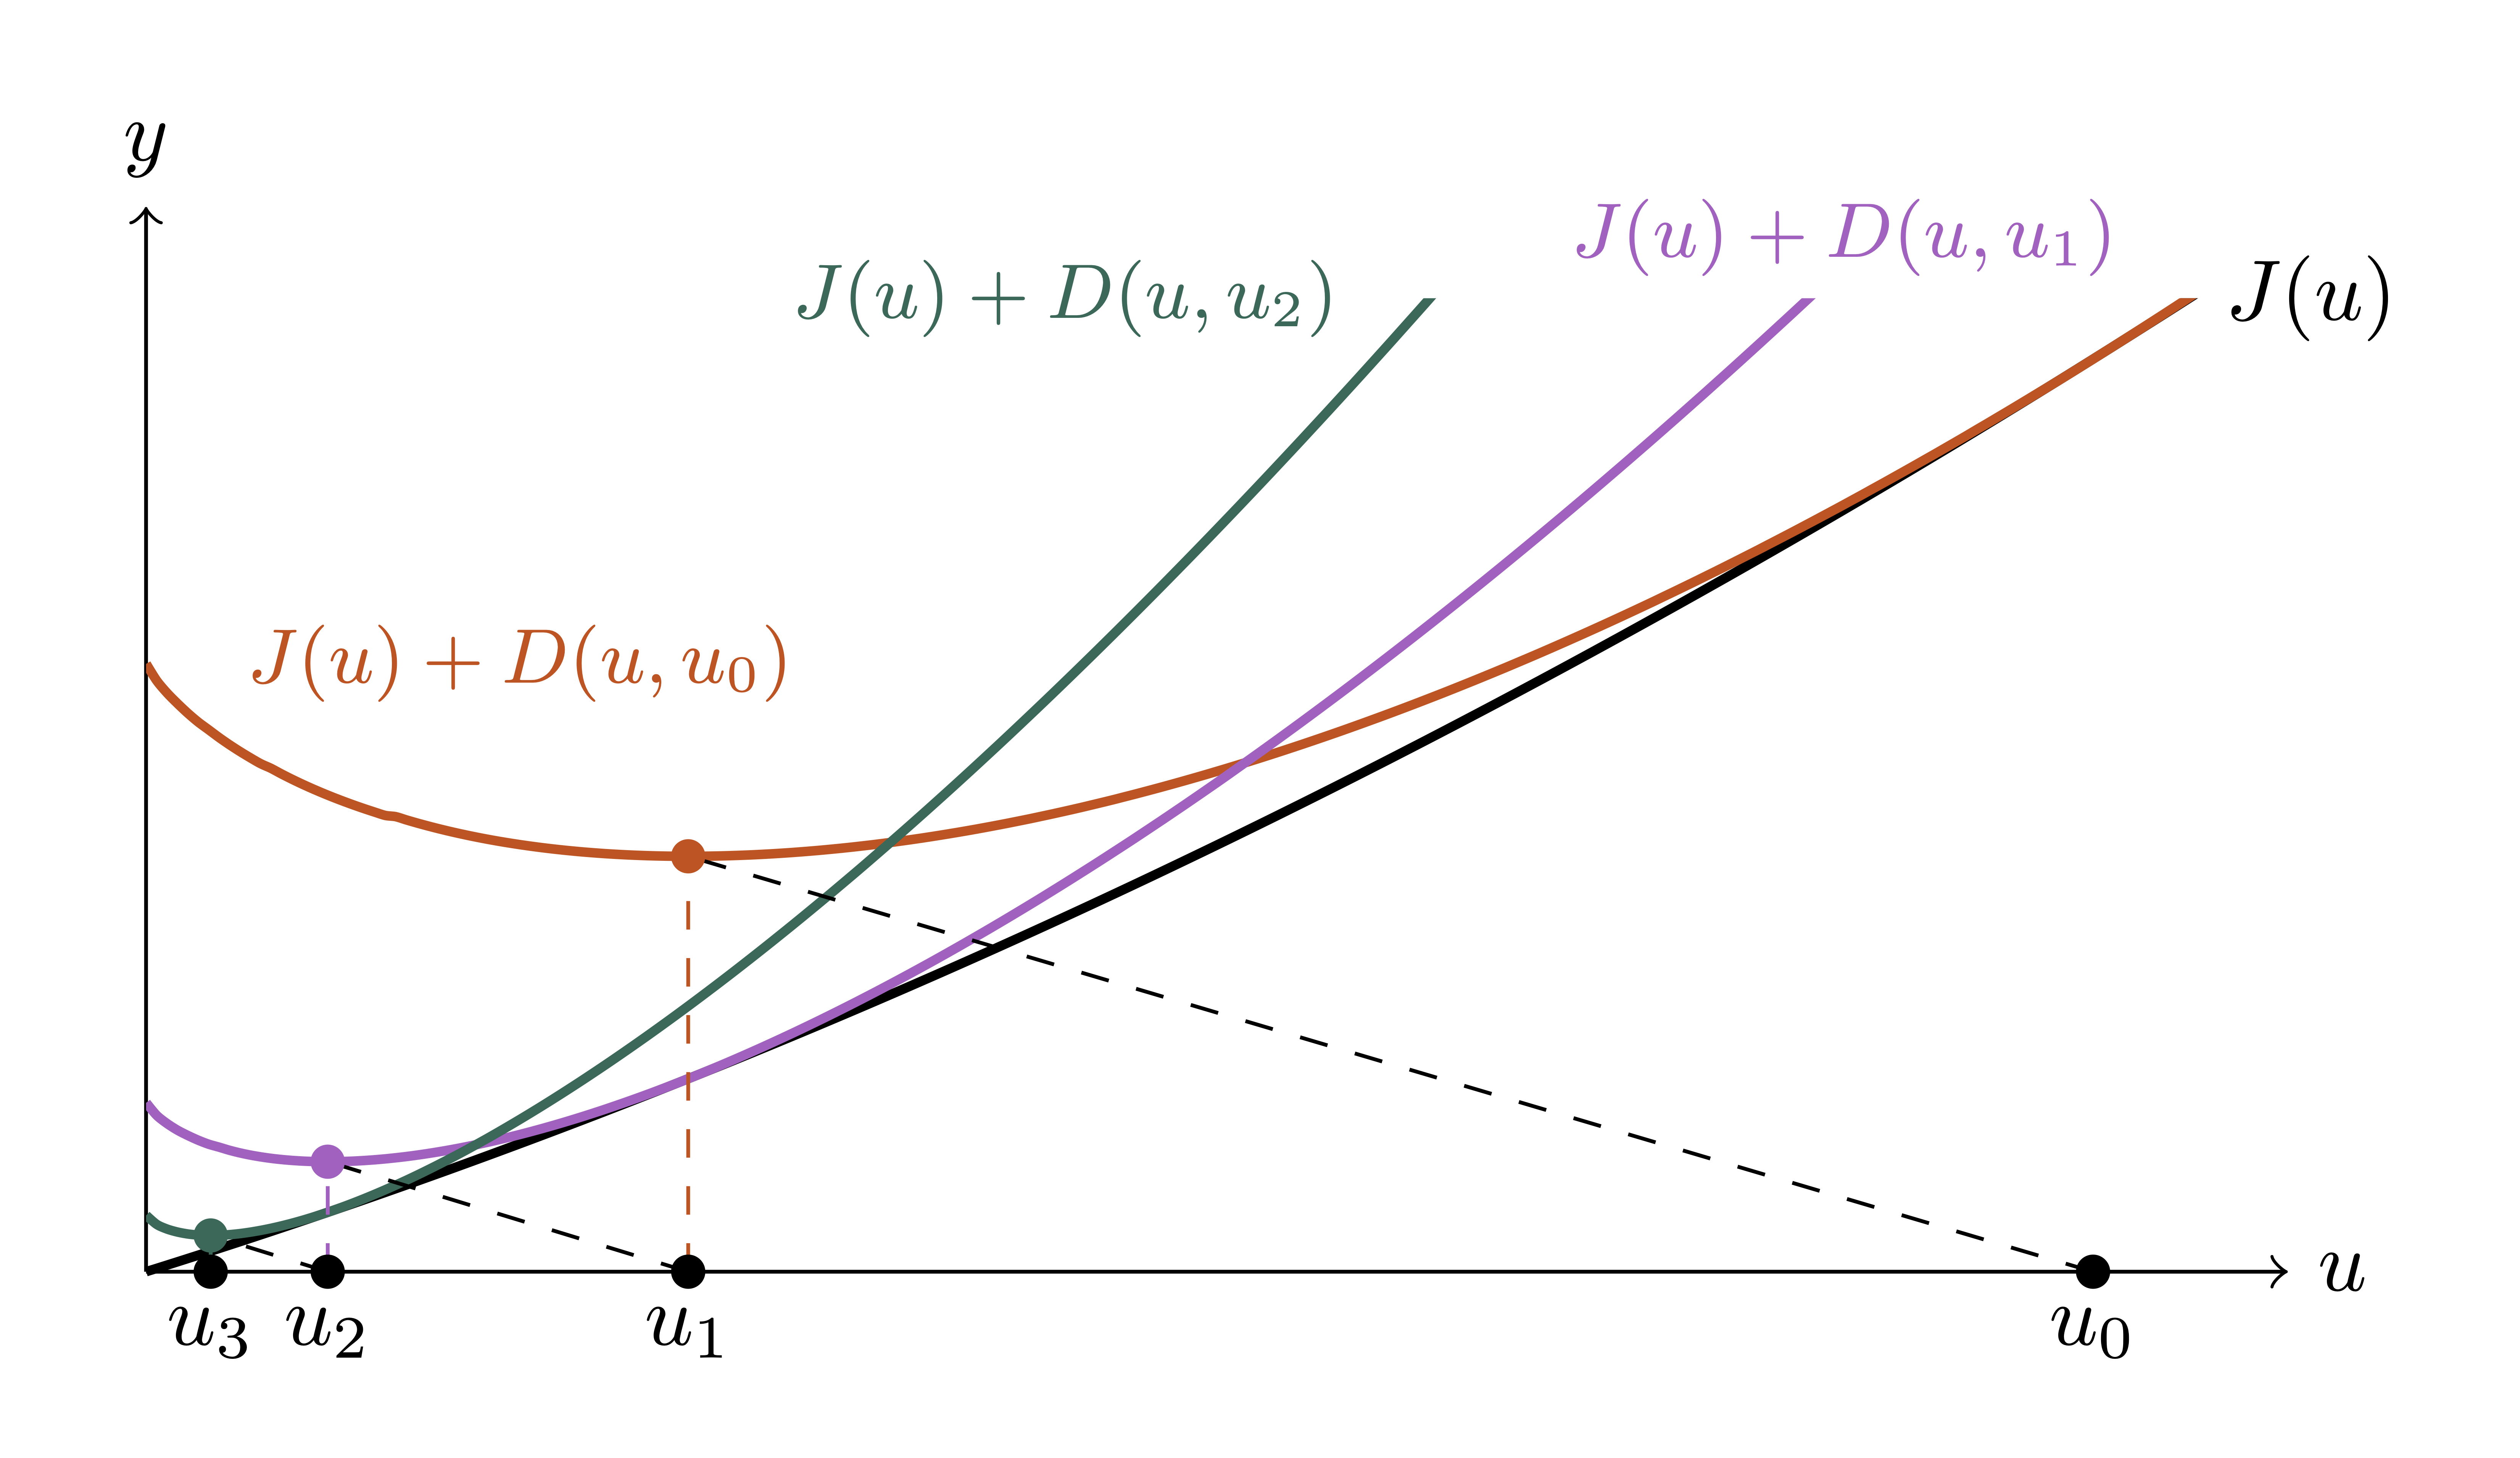
\includegraphics[width=0.8\linewidth]{figures/Prox.png}
\caption{Illustration of Bregman Proximal Point.} 
\end{figure}
\end{minipage}
}
\end{frame}

\begin{frame}\frametitle{Bregman Distances}

\begin{minipage}{0.5\linewidth}
\begin{beamercolorbox}[rounded=true, shadow=true, wd=\textwidth]{block body}
\visible<1->{Bregman distances/divergences are induced by \textbf{distance-generating functions} $R$.}\smallskip

\visible<2->{They measure the linearization error of $R$:
\begin{equation*}
%\label{eq:BregmanDivergence}
D_R(a, b) := R(a) - R(b) - \nabla R(b) \cdot (a-b),
\end{equation*}
for all $a \in \mathop{\text{dom}} R,~b \in \mathop{\text{int}} \mathop{\text{dom}} R$.}
\end{beamercolorbox}
\end{minipage}\visible<2->{
 \begin{minipage}{0.4\linewidth}
 \centering
\begin{figure}[h]
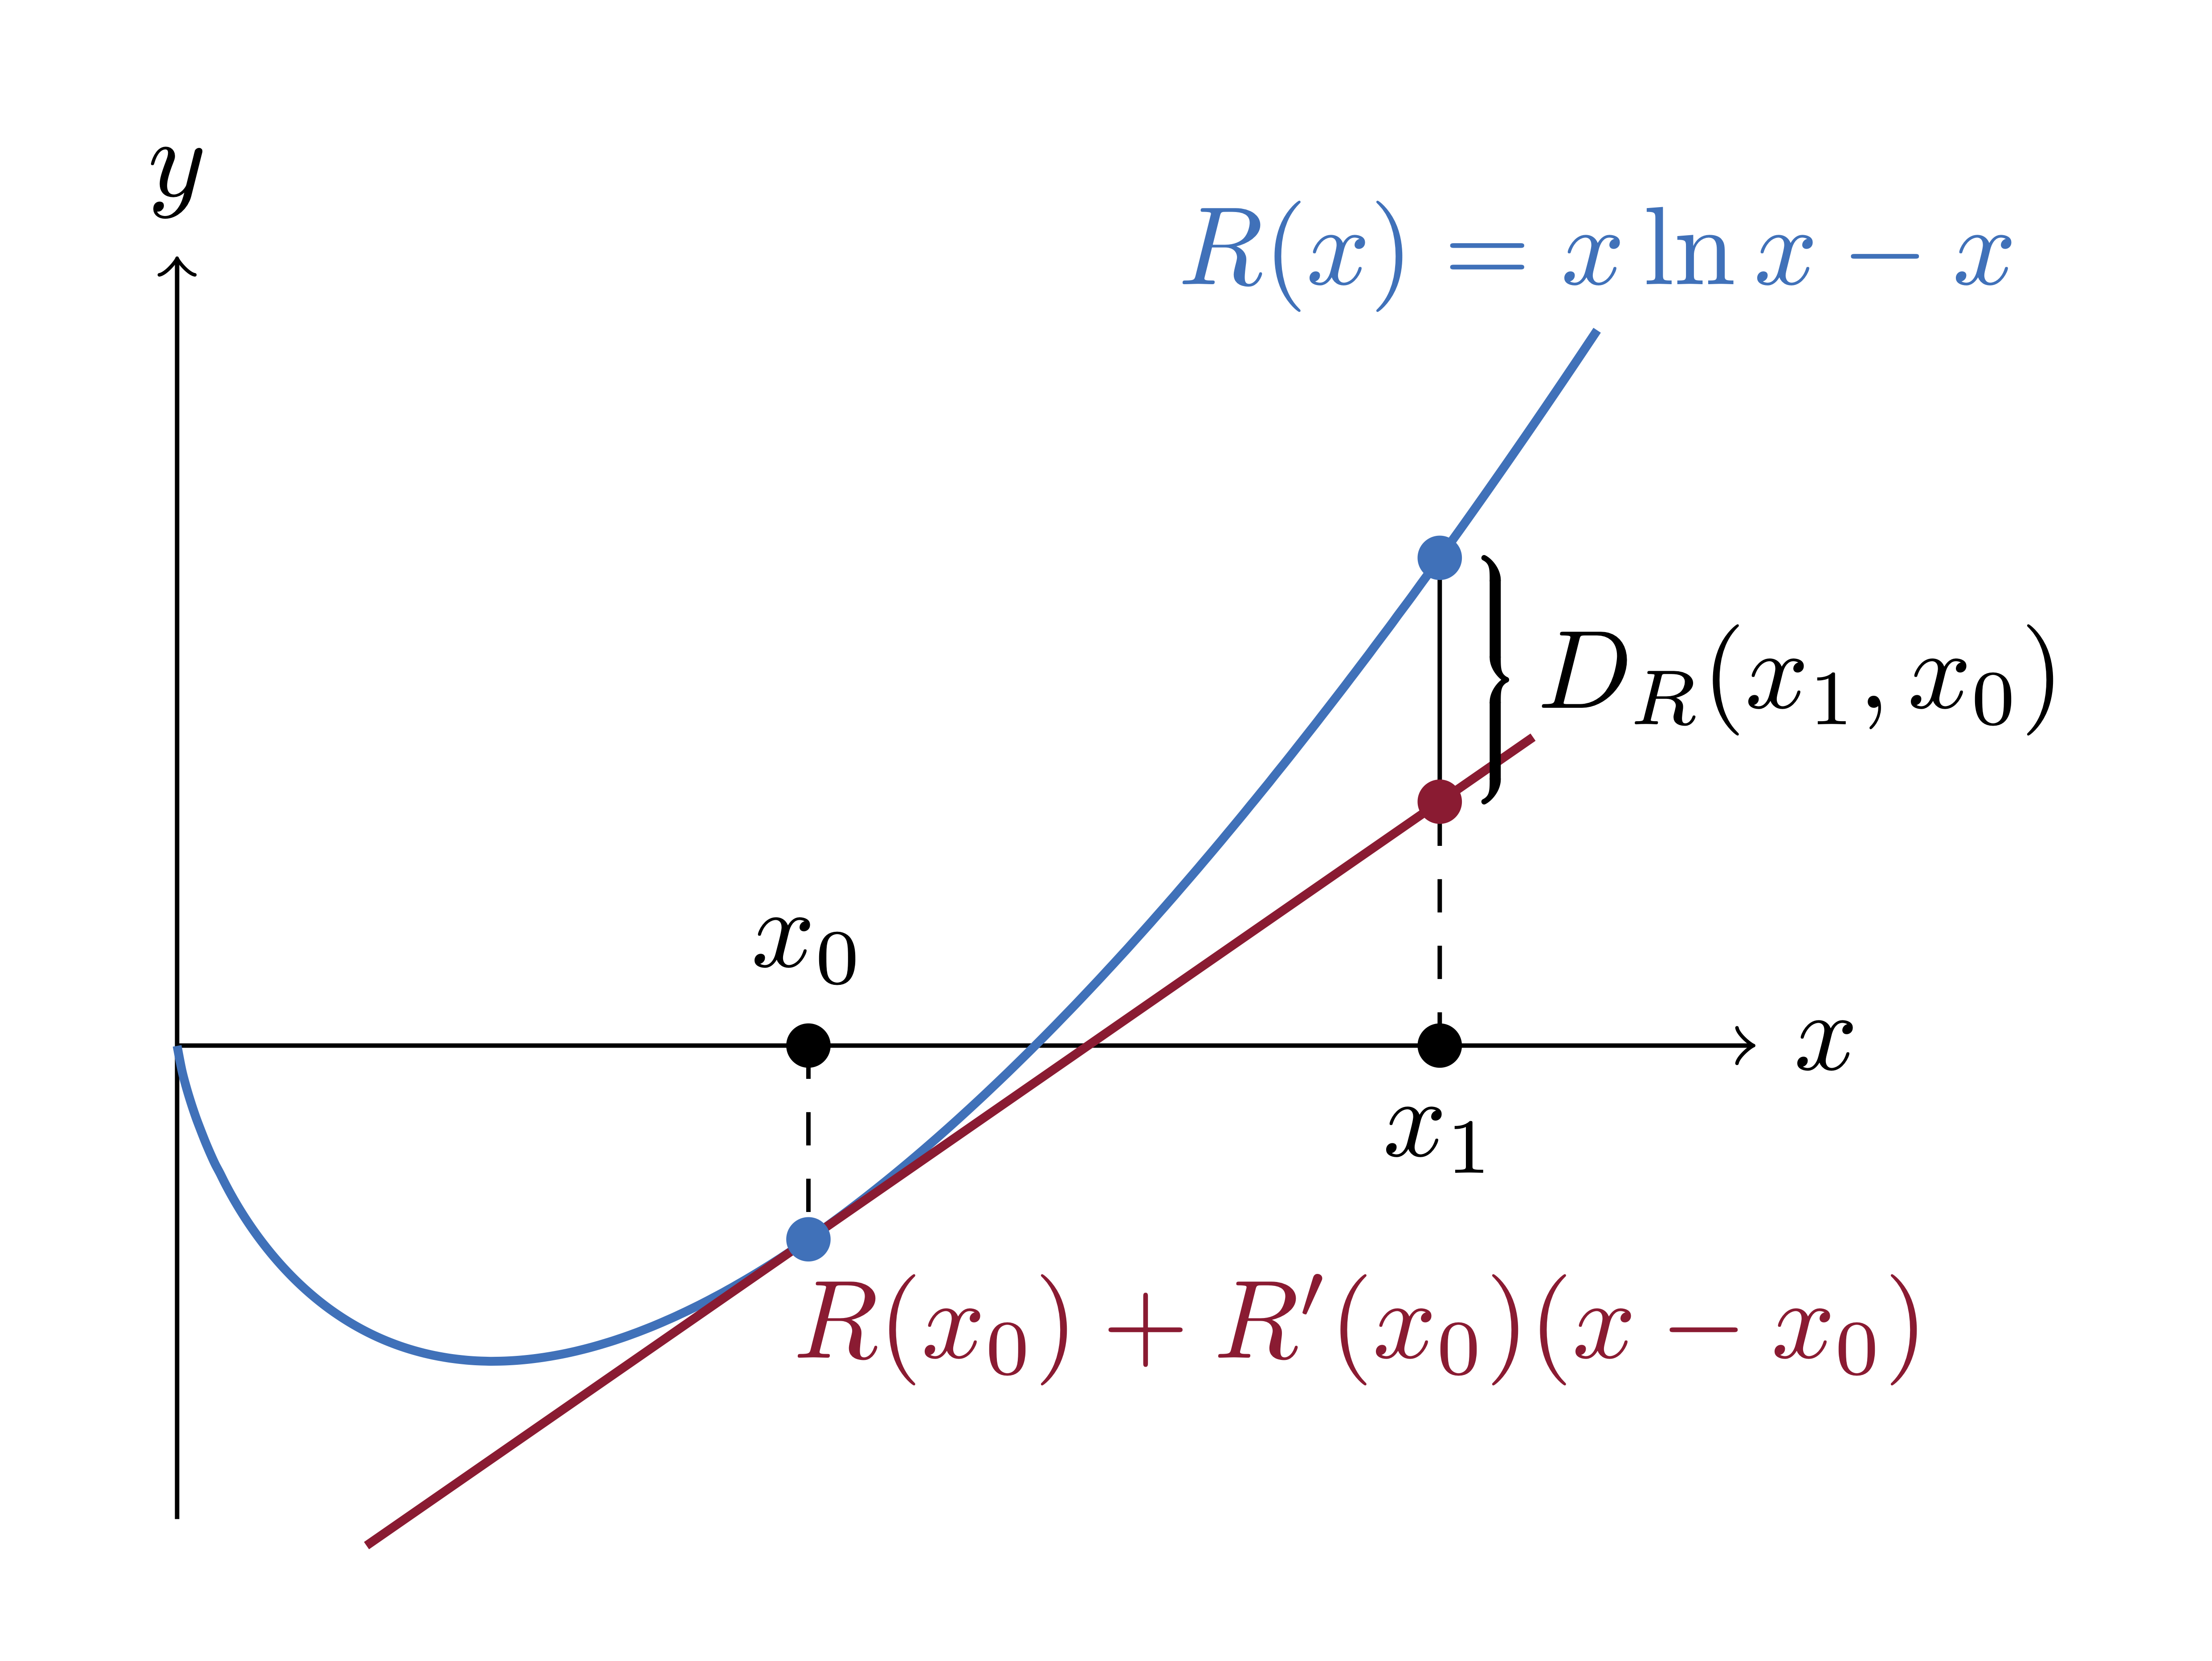
\includegraphics[width=0.8\linewidth]{figures/Bregman.png}
\end{figure}}
\visible<3->{
\begin{beamercolorbox}[rounded=true, shadow=true, wd=\textwidth]{block title}
They are very useful when the geometry of $K$ can be encoded in $\mathop{\text{dom}} R$.
\end{beamercolorbox}}
\end{minipage}
\end{frame}

\begin{frame}\frametitle{Observations}
\begin{beamercolorbox}[rounded=true, shadow=true, wd=\textwidth]{block title}
\centering
 \visible The abstract LVPP framework lies in the construction of the Bregman divergence.
\end{beamercolorbox}

\visible<2->{
\begin{beamercolorbox}[rounded=true, shadow=true, wd=\textwidth]{block body}
Minimal properties of $R$:
\begin{itemize}
\item \visible<2->{Proper: $R > -\infty$ and there exists $a \in \mathbb R^n$ such that $R(a) < +\infty$.\smallskip}

\item \visible<3->{Convex: $R(\lambda a + (1-\lambda)b) \le \lambda R(a) + (1-\lambda) R(b) \quad \forall a,b \in \mathbb R^n, \forall \lambda \in [0,1]$.\smallskip}

\item \visible<4->{Lower semicontinuous: $\forall a \in \mathbb R^n$ ($\{a_n\} \subset \mathbb R^n : a_n \to a \Rightarrow \liminf_{n} R(a_n) \ge R(a)$).\smallskip}

\item \visible<5->{Differentiable in the interior of the effective domain of $R$.}
\end{itemize}
\end{beamercolorbox}}
\visible<6->{
\begin{beamercolorbox}[rounded=true, shadow=true, wd=\textwidth]{block body}
$D_{R}$ is a not a metric, but still: $D_{R}(a,b) = R(a) - R(b) - \nabla R(b)(a-b) \ge 0$.
%\begin{multline*}
%\visible<7->{R(\lambda a + (1-\lambda)b) \le \lambda R(a) + (1-\lambda) R(b)}\visible<8->{ \Rightarrow
%R(b + \lambda (a-b)) - R(b) \le \lambda (R(a)  - R(b))}\visible<9->{ \Rightarrow\\
%\lambda^{-1}(R(b + \lambda (a-b)) - R(b)) \le R(a) - R(b)}\visible<10->{ \Rightarrow
%R(a) - R(b) - \nabla R(b)(a-b) \ge 0.}
%\end{multline*}
\end{beamercolorbox}
}
\end{frame}

%\begin{frame}\frametitle{Legendre Functions}
%\begin{itemize}
%\item Recall what we did with Bregman proximal point and use the graphic from the Austin talk
%\item The key to developing an abstract LVPP framework for more general constraints lies in the way we construct the Bregman divergence.
%\item As you may recall, the Bregman divergence gives us the linearization error of a particular type of proper, convex, lower-semicontinuous function $R$
%\item The Bregman divergence is not symmetric, but it is always non-negative on its domain.
%\item We will now take a deeper look at an important class of convex functions called \alert{Legendre functions}
%\end{itemize}
%\end{frame}

\begin{frame}[plain,c]
%\frametitle{A first slide}
\hfill
\begin{center}
\Huge What are some \alert{relevant} distance-generating functions?
\end{center}
\hfill
\end{frame}

\begin{frame}\frametitle{The Convex Conjugate\footnote{\tiny Also called: Legendre-Fenchel Transform, Dual Function, Fenchel Conjugate}}
  \begin{minipage}{0.67\linewidth}
\begin{beamercolorbox}[rounded=true, shadow=true, wd=\textwidth]{block body}
 Let $X$ be a real topological vector space and $X^*$ its topological dual with pairing denoted by $\langle \cdot,\cdot \rangle$. 
 Given $f: X \to \overline{\mathbb R}$, its \alert{convex conjugate} is the function $f^* : X^* \to \overline{\mathbb R}$ defined by
 \[
 f^*(x^*) := \sup_{x \in X} \left\{\langle x^*,x\rangle - f(x) \right\}.
 \]
\end{beamercolorbox}
\end{minipage}\hfill
\begin{minipage}{0.3\linewidth}
 \centering
 \begin{figure}
  \centering\vspace{1ex}
  \visible<1->{\begin{minipage}[b]{0.45\textwidth}
    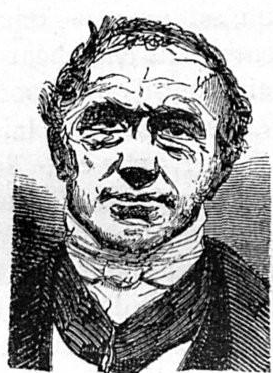
\includegraphics[width=\linewidth]{figures/legendre.png}
    \captionof*{figure}{\tiny A-M. Legendre}
  \end{minipage}}%
  \hfill
  \begin{minipage}[b]{0.46\textwidth}
    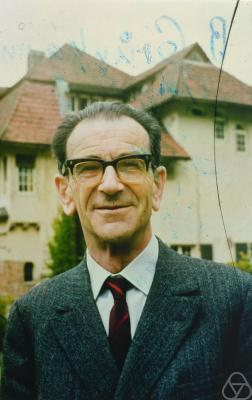
\includegraphics[width=\linewidth]{figures/Werner_Fenchel.jpeg}
    \captionof*{figure}{\tiny W. Fenchel}
  \end{minipage}
\end{figure}

\end{minipage}
\begin{beamercolorbox}[rounded=true, shadow=true, wd=\textwidth]{block title}\centering
$f^*$ is convex (prove this), but it may be nowhere finite.
\end{beamercolorbox}
\end{frame}

\begin{frame}[plain,c]
\centering
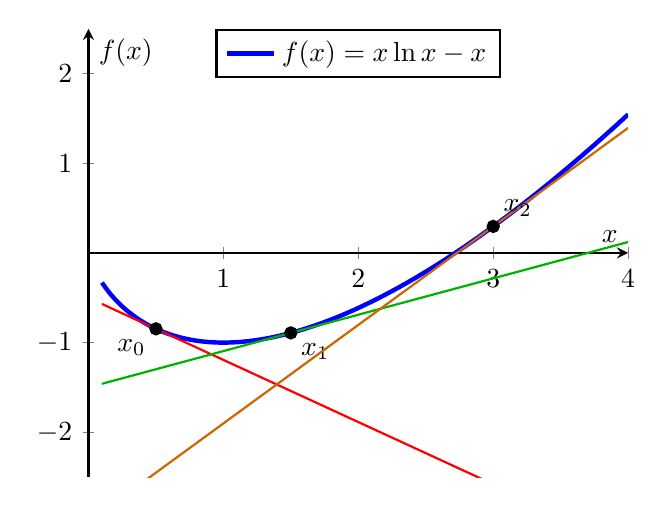
\begin{tikzpicture}
  \begin{axis}[
      axis lines=middle,
      xlabel={$x$},
      ylabel={$f(x)$},
      domain=0.1:4,
      samples=200,
      ymin=-2.5, ymax=2.5,
      xmin=0, xmax=4,
      legend style={at={(0.5,1.0)}, anchor=north},
      thick
    ]
    
    % Function
    \addplot[blue, ultra thick, domain=0.1:4] {x*ln(x) - x};
    \addlegendentry{$f(x) = x \ln x - x$}
    
    % Tangents at x0, x1, x2
    % x0 = 0.5
    \pgfmathsetmacro\xA{0.5}
    \pgfmathsetmacro\yA{\xA*ln(\xA) - \xA}
    \pgfmathsetmacro\mA{ln(\xA)}
    \addplot[red,  thick, domain=0.1:4] {\mA*(x - \xA) + \yA};
    \addplot[only marks, mark=*] coordinates {(\xA,\yA)};
    \node[below left] at (axis cs:\xA,\yA) {$x_0$};

    % x1 = 1.5
    \pgfmathsetmacro\xB{1.5}
    \pgfmathsetmacro\yB{\xB*ln(\xB) - \xB}
    \pgfmathsetmacro\mB{ln(\xB)}
    \addplot[green!70!black,  thick, domain=0.1:4] {\mB*(x - \xB) + \yB};
    \addplot[only marks, mark=*] coordinates {(\xB,\yB)};
    \node[below right] at (axis cs:\xB,\yB) {$x_1$};

    % x2 = 3.0
    \pgfmathsetmacro\xC{3.0}
    \pgfmathsetmacro\yC{\xC*ln(\xC) - \xC}
    \pgfmathsetmacro\mC{ln(\xC)}
    \addplot[orange!80!black,  thick, domain=0.1:4] {\mC*(x - \xC) + \yC};
    \addplot[only marks, mark=*] coordinates {(\xC,\yC)};
    \node[above right] at (axis cs:\xC,\yC) {$x_2$};

  \end{axis}
\end{tikzpicture}\vspace{2ex}
\begin{beamercolorbox}[rounded=true, shadow=true, wd=\textwidth]{block title}\centering
$f^*$ encodes all the information of the convex hull of $f(x)$'s epigraph in terms of its supporting hyperplanes.
\end{beamercolorbox}
\end{frame}

\begin{frame}\frametitle{An Example}
\begin{example}
Let $f(x) = \exp x$. Then $f: \mathbb R \to \mathbb R$ and $f^* : \mathbb R \to \overline{\mathbb R}$ is given by
\[
f^*(x^*) := \sup_{x \in \mathbb R}\{ x^* x - \exp(x) \} = - \inf_{x \in \mathbb R}\{\exp(x) - x^* x\}.
\]
\visible<2->{If $x^* < 0$, then $x\to -\infty$ implies $x^* x - \exp(x) \to +\infty$. Hence, $f^*(x^*) = +\infty$. \medskip}

\visible<3->{If $x^* = 0$, then the least upper bound of $-\exp(x)$ over $x \in \mathbb R$ is 0. Hence, $f^*(x^*) = 0$.  \medskip}

\visible<4->{If $x^* > 0$, then the minimizer of $\exp(x) - x^*x$ solves $\exp(x) = x^*$, i.e., $x = \ln(x^*)$. \medskip}

\visible<5->{So the \alert{convex conjugate} of \alert{$f(x) = \exp(x)$} is Shannon's entropy extended to $\mathbb R$.}
\end{example}
\end{frame}

\begin{frame}\frametitle{The Hellinger Entropy}
\begin{example}
Let $f(x) = -\sqrt{1 - \|x\|^2}$ with $f(x) = +\infty$ for $\|x\| > 1$. Here, we have for $\|x\| \le 1$
\[ 
(\langle x^*, \cdot\rangle - f(\cdot))'(x) = x^* -  (1 - \|x\|^2)^{-1/2} x \Rightarrow x(x^*) = \frac{x^*}{\sqrt{1 + \|x^*\|^2}}
\]
By substitution, we get
\[
f^*(x^*) = \frac{1 + \|x^*\|^2}{\sqrt{1 + \|x^*\|^2}}.
\]
Note: 
\[
\nabla f^*(x^*) = \frac{x^*}{\sqrt{1 + \|x^*\|^2}} \text{ and } \| \nabla f^*(x^*) \| \le 1.
\]
\end{example}
\end{frame}

\begin{frame}\frametitle{Observation}
\begin{beamercolorbox}[rounded=true, shadow=true, wd=\textwidth]{block body}
Given $R_1(a) := a \ln a - a$ and $R_2(a) := -\sqrt{1 - \|a\|^2}$ we see that 
\[
R_1^*(a^*) = \exp(a^*) \text{ and } R_2(a^*) = \frac{1 + \|a^*\|^2}{\sqrt{1 + \|a^*\|^2}}.
\]\visible<2->{
Moreover, though $R_1$, $R_2$ have restricted domains, $R^*_1$, $R^*_2$ are defined on all of $\mathbb R^n$.\medskip}

\visible<3->{What's more: $\nabla R^*_1(a^*) = \exp(a^*)$ and $\nabla R^*_2(a^*) =  \frac{a^*}{\sqrt{1 + \|a^*\|^2}}$}\visible<3->{ and 
\[
\nabla R^*_1(\mathbb R) \subset \mathrm{int \, dom\,} R_1 \text{ and } \nabla R^*_2(\mathbb R^n) \subset \mathrm{int \, dom\,} R_2.
\]}\vspace{-2ex}
\end{beamercolorbox}

\visible<5->{
\begin{beamercolorbox}[rounded=true, shadow=true, wd=\textwidth]{block body}\centering
Is there are general class of functions $R$ for which $\nabla R^*$ maps into  $\mathrm{int \, dom\,} R$? \alert{Yes!}.
\end{beamercolorbox}}
\end{frame}

\begin{frame}\frametitle{Legendre Functions\footnote{\tiny Originally introduced by Rockafellar in 1967, we follow the definition and nomenclature of Teboulle (2018)}}

\visible<1->{
\begin{beamercolorbox}[rounded=true, shadow=true, wd=\textwidth]{block body}\centering
The geometry of a closed convex set $C \subset \mathbb{R}^m$ with a non-empty interior, $\operatorname{int}C \neq \emptyset$, can be encoded into a \alert{Legendre function} $R: \mathbb{R}^m \to \mathbb{R}\cup\{+\infty\}$.
\end{beamercolorbox}}

\begin{minipage}{0.7\textwidth}
\begin{definition}[]
%\label{def:LegendreFunction}
\visible<2->{
Let the essential domain of a function $R$ be defined as $\operatorname{dom} R := \{ a \in \mathbb{R}^m \mid R(a) < \infty \}$.
}\visible<3->{We call a proper convex function a \alert{Legendre function} $R: \mathbb{R}^m \to \mathbb{R}\cup\{+\infty\}$ if}
\begin{itemize}
%% \itemsep=-3pt
\item \visible<4->{$\operatorname{int}(\operatorname{dom} R) \neq \varnothing$;}
\item \visible<5->{$R$ is differentiable on $\operatorname{int}(\operatorname{dom} R)$;}
\item \visible<6->{$\lim_{t \to 0^+} \langle \nabla R(a+t(b-a)), b-a\rangle = -\infty$ for all $a \in \partial( \operatorname{dom} R)$ and $b \in \operatorname{int}(\operatorname{dom} R)$;}
\item \visible<7->{R is strictly convex on $\operatorname{int}(\operatorname{dom} R)$.}
\end{itemize}
\end{definition}
\end{minipage}\hfill
\begin{minipage}{0.3\linewidth}
 \centering
 \begin{figure}
  \centering\vspace{1ex}
  \begin{minipage}[b]{0.6\textwidth}
    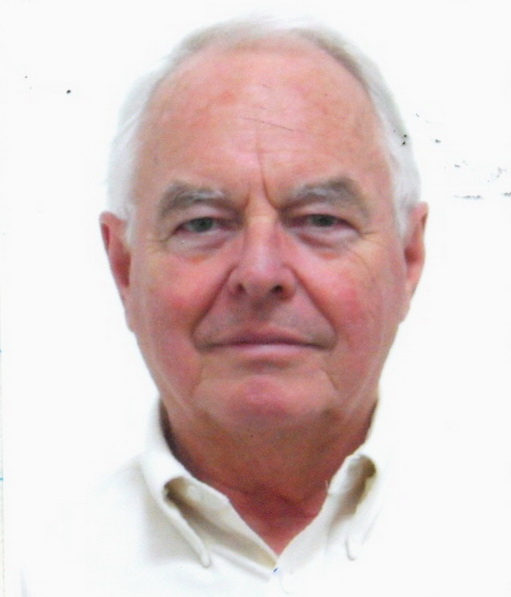
\includegraphics[width=\linewidth]{figures/rtr.jpg}
    \captionof*{figure}{\tiny R. Tyrrell Rockafellar}
  \end{minipage}%
  \end{figure}
  \end{minipage}



%Introduced by Rockafellar in 1967~\cite{Rockafellar1967Conjugates}, see also \cite[Chap.~26]{RTRockafellar_1970}, Legendre functions constitute a special class of proper convex functions whose gradients $\nabla R$ become singular on the boundary of their essential domains.
%We denote by $R^*(a^\ast) \coloneqq \sup \{ a \cdot a^\ast - R(a) \mid a \in \mathbb{R}^m \}$ the convex conjugate of $R$.
%
%\begin{theorem}[Rockafellar \text{\cite[Thm. 1]{Rockafellar1967Conjugates}}]
%\label{thm:Rockafellar}
%A proper convex function $R$ is a Legendre function if and only if its convex conjugate $R^\ast$ is also a Legendre function.
%Moreover, $\nabla R \colon \operatorname{int}(\operatorname{dom} R) \to \operatorname{int}(\operatorname{dom} R^*)$ is a topological isomorphism with $(\nabla R)^{-1} = \nabla R^\ast$.
%\end{theorem}
%
%
%From now on, we assume that ${R(a)}/{|a|} \to +\infty$ as $|a| \to \infty$ and $\operatorname{dom} R = C$.
\end{frame}

\begin{frame}\frametitle{Properties of Legendre Functions}

\visible<1->{
\begin{beamercolorbox}[rounded=true, shadow=true, wd=\textwidth]{block body}\centering
 Legendre functions constitute a special class of proper convex functions whose gradients $\nabla R$ become singular on the boundary of their essential domains.
\end{beamercolorbox}}

\begin{minipage}{0.7\textwidth}
\begin{theorem}[Rockafellar (1967)]
\label{thm:Rockafellar}
A proper convex function $R$ is a Legendre function if and only if its convex conjugate $R^\ast$ is also a Legendre function.
Moreover, $\nabla R \colon \operatorname{int}(\operatorname{dom} R) \to \operatorname{int}(\operatorname{dom} R^*)$ is a topological isomorphism with $(\nabla R)^{-1} = \nabla R^\ast$.
\end{theorem}
\end{minipage}\hfill
\begin{minipage}{0.3\linewidth}
 \centering
 \begin{figure}
  \centering\vspace{1ex}
  \begin{minipage}[b]{0.6\textwidth}
    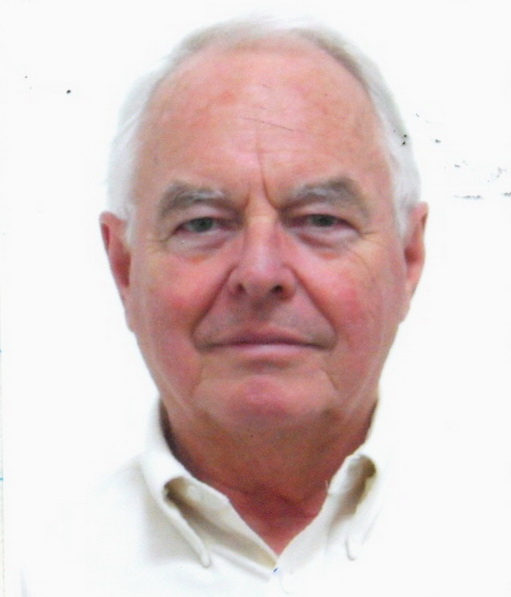
\includegraphics[width=\linewidth]{figures/rtr.jpg}
    \captionof*{figure}{\tiny R. Tyrrell Rockafellar}
  \end{minipage}%
  \end{figure}
  \end{minipage}

\visible<2->{
\begin{beamercolorbox}[rounded=true, shadow=true, wd=\textwidth]{block title}\centering
It can also be shown that ${R(a)}/{|a|} \to +\infty$ as $|a| \to \infty$ if and only if $\operatorname{dom} R^* = \mathbb R^n$.
\end{beamercolorbox}}

\end{frame}

\begin{frame}\frametitle{Geometry Preserving Transformations}

\begin{beamercolorbox}[rounded=true, shadow=true, wd=\textwidth]{block title}
\begin{equation*} \label{eq:intro:feasible_set}
K = \{ v \in V \mid Bv(x) \in C(x) \text{ for almost every } x \in \Omega_d \subset \overline{\Omega} \}.
\end{equation*}
\end{beamercolorbox}\hfill

\begin{minipage}{0.5\linewidth}
\begin{beamercolorbox}[rounded=true, shadow=true, wd=\textwidth]{block title}
\centering
 $\nabla R \colon \operatorname{int}C \to \operatorname{int}(\operatorname{dom} R^*)$ satisfies %is a topological isomorphism 
 $(\nabla R)^{-1} = \nabla R^\ast$
\end{beamercolorbox}
\end{minipage}
%
\begin{minipage}{0.4\linewidth}
\begin{figure}[h]
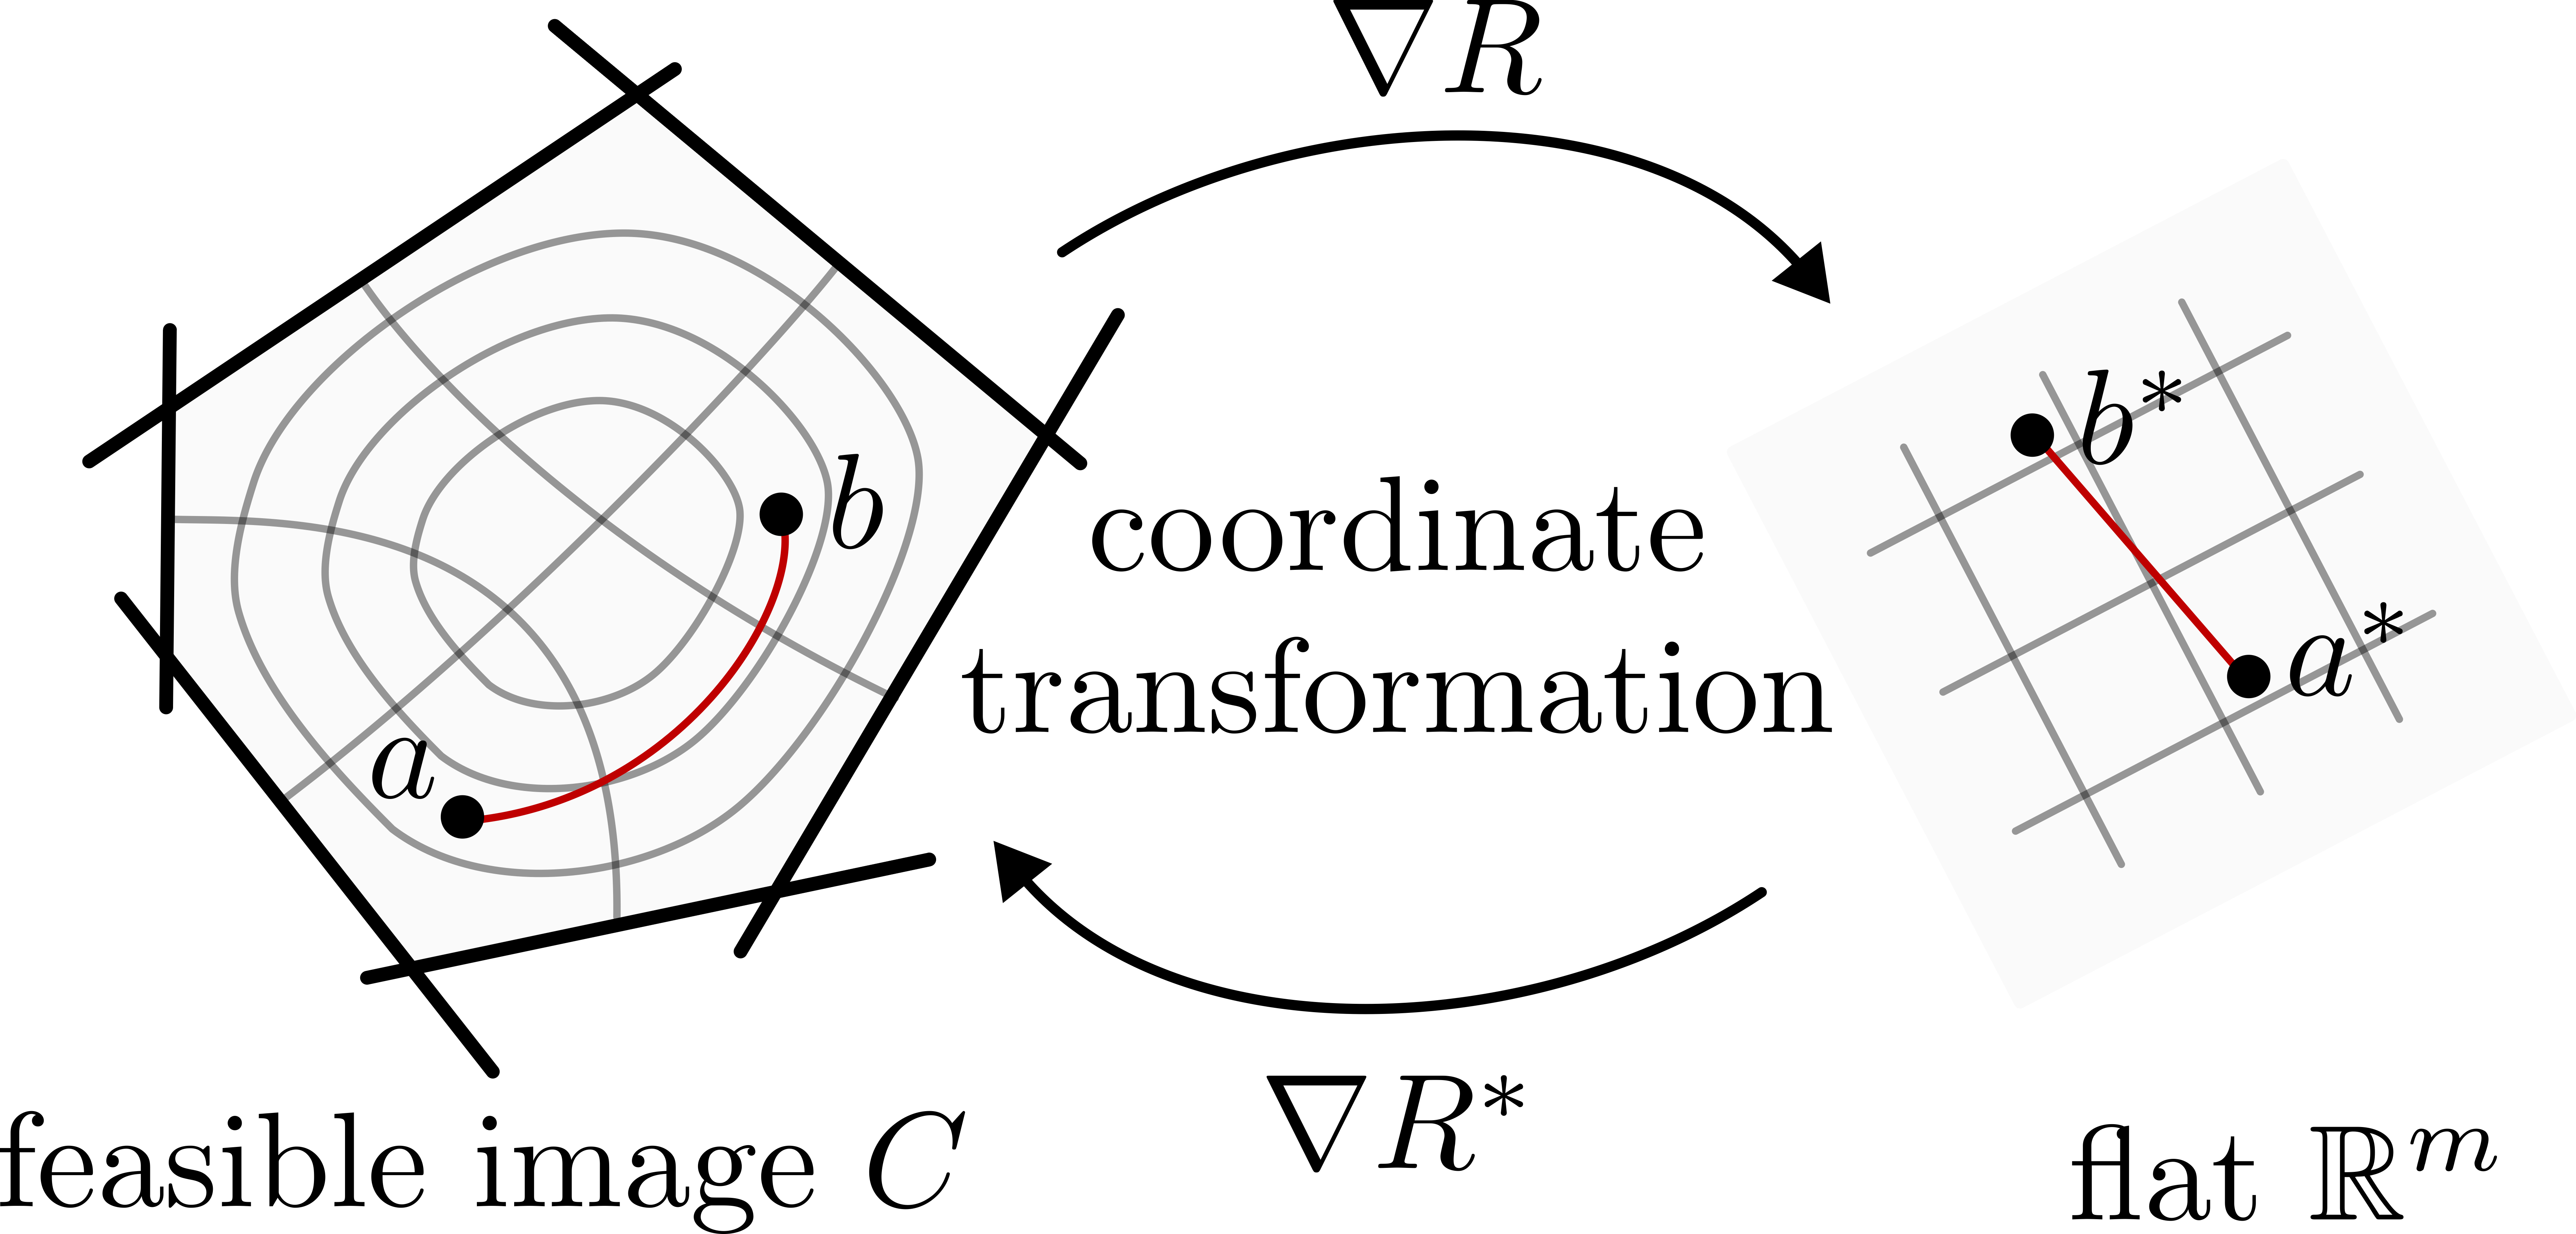
\includegraphics[width=0.8\linewidth]{figures/Geodesic3.png} 
\end{figure}
\end{minipage}
\end{frame}


\begin{frame}[plain,c]
%\frametitle{A first slide}
\hfill
\begin{center}
\Large With the help of Legendre functions, we can find mappings that \alert{guarantee} feasibility for pointwise inequality constraints.
\end{center}
\hfill
\end{frame}

\begin{frame}\frametitle{}
\thispagestyle{empty}
%\hypertarget{lvpp-table}{}
%\hyperlink{lvpp-examples}{\beamerbutton{Go to Examples}}
\begin{table}
\centering
\small
% \renewcommand{\arraystretch}{0.6}
\setlength{\tabcolsep}{5pt}
\renewcommand{\arraystretch}{1.4}
    \begin{tabular}{ c|c|c|c } 
     \toprule
      Feasible set $K$ & Legendre function $R$ & $B$ & $\nabla R^*(\psi)$ \\ 
     \midrule
     $\big\{ u \geq \phi \big\}$ & $(a - \phi) \ln (a - \phi) - (a - \phi)$ & $\operatorname{id}$ & $\phi + \exp\psi$ \\[2ex]
     $\big\{ \phi_1 \leq u \leq \phi_2 \big\}$ & $(a - \phi_1) \ln (a - \phi_1) + (\phi_2-a) \ln (\phi_2-a)$ & $\operatorname{id}$ & $\dfrac{\phi_1 + \phi_2\exp\psi}{1 + \exp\psi}$ \\[2ex]
     % $\big\{ \phi_1 \leq u \leq \phi_2 \big\}$ & $\sum_{i=1}^2 (-1)^i (\phi_i - a) \ln \left( (-1)^i (\phi_i - a)\right)$ & $\operatorname{id}$ & $\dfrac{\phi_1 + \phi_2\exp\psi}{1 + \exp\psi}$ \\[2ex]
     $\big\{\gamma u \ge \phi \big\}$ & $(a-\phi) \ln (a - \phi) - (a - \phi)$ & $\gamma$ &  $\phi + \exp\psi$ \\[2ex]
     $\big\{ (\gamma u)\cdot n \leq \phi \big\}$ & $(\phi-a) \ln (\phi - a) - (\phi - a)$ & $\gamma(\cdot) \cdot n$ & $\phi - \exp(-\psi)$ \\[2ex]
     $\big\{| \nabla u | \le \phi \big\}$ & $ -\sqrt{\phi^2 - | a |^2}$ & $\nabla$  & $\dfrac{\phi\psi}{\sqrt{1 + | \psi |^2}}$ \\[3ex] 
     $\big\{ u \ge 0,\; \sum_{i} u_i = 1 \big\}$ & $\sum_{i} a_i \ln(a_i)$ & $\operatorname{id}$ & $\dfrac{\exp\psi}{\sum_{i} \exp\psi_i}$\\[2ex]
     $\big\{ \det (\nabla^2 u) \geq 0 \big\}$ & $\operatorname{tr}(a\ln a - a)$ & $\nabla^2$ & $\exp \psi$ \\[2ex]
     \bottomrule
    \end{tabular}
\vspace{-1em}
%\end{sidewaystable}
\end{table}
\end{frame}

\begin{frame}\frametitle{A}
\begin{itemize}
%\item Define proper, convex, lsc again
%\item Define convex conjugate and motivate its meaning
%\item Define Legendre function
%\item Find a picture of Rockafellar
%\item Work out two examples to show how to compute the convex conjugate
%\item Prove (if possible) the crucial Rockafellar theorems
%\item Give the table in the paper
\item Return to Bregman 
\end{itemize}
\end{frame}

\begin{frame}\frametitle{A}
\begin{itemize}
\item
\end{itemize}
\end{frame}

\begin{frame}\frametitle{A}
\begin{itemize}
\item
\end{itemize}
\end{frame}

\begin{frame}\frametitle{A}
\begin{itemize}
\item
\end{itemize}
\end{frame}

\begin{frame}\frametitle{A}
\begin{itemize}
\item
\end{itemize}
\end{frame}

\begin{frame}\frametitle{A}
\begin{itemize}
\item
\end{itemize}
\end{frame}

\section{The General LVPP Algorithm}
\begin{frame}\frametitle{A}
\begin{itemize}
\item
\end{itemize}
\end{frame}

\section{Applications}
\begin{frame}\frametitle{A}
\begin{itemize}
\item
\end{itemize}
\end{frame}

\end{document}